% Template: đường tròn (O), một điểm M ngoài đường tròn, hai tiếp tuyến MA, MB.
% Tiếp điểm A, B đối xứng qua OM. Tính sẵn theo công thức:
%   Đặt OM = d, R = bán kính. Khi đó OA vuông góc MA, |OA| = R, |MA| = sqrt(d^2 - R^2).
\documentclass[border=5pt]{standalone}
\usepackage{tikz}
\usetikzlibrary{calc,intersections,through}
\begin{document}
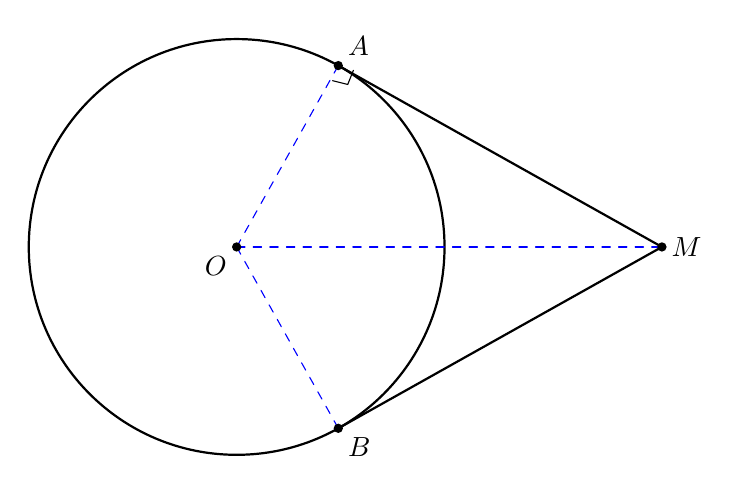
\begin{tikzpicture}[scale=1.2, line cap=round, line join=round]
  \def\R{2.2}      % bán kính
  \def\d{4.5}      % khoảng cách OM

  \coordinate (O) at (0,0);
  \coordinate (M) at (\d,0);

  % Tiếp điểm: A, B trên đường tròn, OA vuông góc AM.
  % Góc giữa OA và OM là alpha với cos(alpha) = R/d.
  \pgfmathsetmacro{\alpha}{acos(\R/\d)}
  \coordinate (A) at (\alpha:\R);
  \coordinate (B) at (-\alpha:\R);

  % Đường tròn (O)
  \draw[thick] (O) circle (\R);

  % Hai tiếp tuyến MA, MB
  \draw[thick] (M) -- (A);
  \draw[thick] (M) -- (B);

  % Bán kính tới tiếp điểm
  \draw[blue, dashed] (O) -- (A);
  \draw[blue, dashed] (O) -- (B);

  % Đoạn OM
  \draw[blue, dashed] (O) -- (M);

  % Ký hiệu vuông góc tại A (giữa OA và AM): hướng tuỳ vào hình, ở đây đặt thủ công.
  \draw ($(A)+(0.16,-0.05)$) -- ($(A)+(0.10,-0.20)$) -- ($(A)+(-0.06,-0.16)$);

  % Chấm điểm
  \foreach \p in {O,M,A,B} \fill (\p) circle (1.4pt);

  % Nhãn
  \node[below left] at (O) {$O$};
  \node[right] at (M) {$M$};
  \node[above right] at (A) {$A$};
  \node[below right] at (B) {$B$};
\end{tikzpicture}
\end{document}
